\documentclass{beamer}

\usepackage[utf8]{inputenc}
\usepackage{graphicx}
\usepackage{multimedia}
\usepackage{url}

\usetheme{default}
\usecolortheme{crane}
\usefonttheme{default}
\useoutertheme{sidebar}
\useinnertheme[shadow=true]{rounded}

\title{Jeu du Pérudo}
\author{H4104 - Dragibus}
\institute{INSA de Lyon}
%\logo{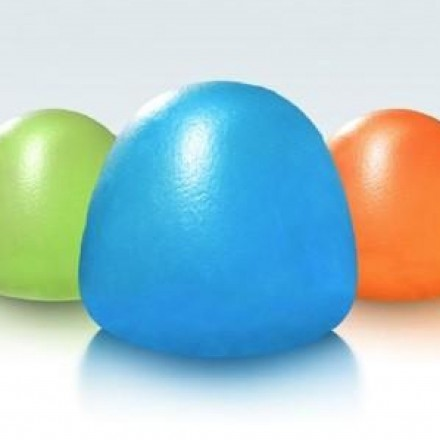
\includegraphics[height=8mm]{logo.jpeg}}

\begin{document}

\begin{frame}
  \titlepage
\end{frame}

\begin{frame}
  \frametitle{Sommaire}
  \tableofcontents[hideallsubsections]
\end{frame}

\section{Mécanisme du jeu}

\begin{frame}
  \frametitle{Principe}

  % TODO intégrer photo du jeu

  \begin{itemize}
    \item jeu de dés
    \item multijoueur, entre 2 et 6 (ou plus) joueurs
    \item deviner le nombre de dés d'une valeur, connaissant seulement ses
      propres dés
    \item dernier joueur ayant des dés gagne la partie
  \end{itemize}
\end{frame}

\begin{frame}
  \frametitle{Règles}
  $\to$ parier sur le nombre de dés en jeu \\
  \emph{(pour une certaine valeur de dé)}

  \begin{itemize}
    \item enchêre
    \item dudo
    \item calza
  \end{itemize}
\end{frame}

\begin{frame}
  \frametitle{Exemple}

  % TODO formatter cette slide

  \begin{center}
    \begin{large}
      Joueur précédent : \textit{"Je pense qu'il y a douze 5"}
      \\
      \uncover<2>{Moi :\textit{"Je pense qu'il y a treize 5"}}
    \end{large}
  \end{center}

  $\to$ la mise ne peut qu'\textbf{augmenter} au cours de la partie
\end{frame}

\section{Concept d'IA}

\begin{frame}
  \frametitle{Constat}

  \begin{large}
    À son tour, le joueur doit \textbf{évaluer} les différents coups possibles.
    \\[1.5cm]
    \begin{center}
      \uncover<2>{\textit{Une IA devrait fonctionner de la même manière.}}
    \end{center}
  \end{large}
\end{frame}

\begin{frame}
  \frametitle{Évaluation}

  \begin{itemize}
    \item état de soi-même (dés)
    \item état du jeu (mise précédente, historique des mises, nombre de dés)
    \item coups possibles
  \end{itemize}

  \center{$ia(EtatJoueur, EtatJeu, CoupsPossibles) \to Evaluation$}
  \\[1cm]
  \large L'IA n'est qu'une \textbf{fonction d'évaluation} de l'état du jeu.
\end{frame}

\begin{frame}
  \frametitle{Combinaison}

  \begin{large}
    Permet de créer des IA complèxes à partir d'autres relativement simples.
    \\[1cm]
    \uncover<2>{Simple combinaison linéaire avec des coefficients de
      \emph{poids}, correspondant à la prise en compte dans la décision
      finale.}
  \end{large}
\end{frame}

\section{Présentation des IA}

\section{Résultats et observations}

\end{document}

% vim: et sw=2 sts=2
